\documentclass[lettersize, noapacite, twoside, HRI]{apa_HRI}


%\usepackage[utf8x]{inputenc}
\usepackage{times}

\usepackage{graphicx} 
\usepackage{subfigure}
\usepackage{paralist}

\usepackage{hyperref}

\usepackage{amsfonts}
\usepackage{mathtools}
\usepackage{url}
\usepackage{xspace}
\usepackage{booktabs}

\usepackage[natbibapa]{apacite}


\usepackage{tikz}
\usetikzlibrary{decorations.pathreplacing}
\newcommand{\tikzmark}[1]{\tikz[overlay,remember picture] \node (#1) {};}

\usepackage[draft,nomargin,footnote]{fixme}

\graphicspath{{figs/}}

\newcommand{\eg}{\textit{e.g.}\xspace}
\newcommand{\etal}{\textit{et al.}\xspace}
\newcommand{\ie}{\textit{i.e.}\xspace}
\newcommand{\etc}{\textit{etc.}\xspace}
\newcommand{\vs}{\textit{vs.}\xspace}

\newcommand{\h}[1]{\textbf{H#1}\xspace}

\newcommand{\anti}{{$\mathcal{A}_0$ }}
\newcommand{\antf}{{$\mathcal{A}_1$ }}
\newcommand{\deltaant}{{ $\Delta_{\mathcal{A}_0,\mathcal{A}_1}$ }}


\rightheader{Impact of Context in the Perception of a Robot}   % This should be the title, or a shortened version of the title if your title is long.
\leftheader{Lemaignan et al.}	  % For one or two authors, include both authors last names.  For three or more, use first author's last name et al.
\title{Impact of Context in the Perception of a Robot}

\author{S\'everin Lemaignan, Ashish Ranjan Jha, Kshitij Sharma, Pierre
Dillenbourg}
\affiliation{CHILI Lab, \'Ecole Polytechnique F\'ed\'erale de Lausanne}

\acknowledgements{\url{firstname.lastname@epfl.ch}}

\abstract{
What leads us to attribute human-like characteristics to robots? The physical
appearance of the robot and the design of its behaviours do obviously play a key
role. This paper however evidences another mechanism at play, more subtle and partially
unconscious: the context of the interaction, and more precisely, the cognitive
prerequisites that the interaction presupposes.

To study this effect, we propose an original methodology based on eye-tracking
and a set of stimuli that are visually identical and yet elicit different
assumptions regarding the cognitive capabilities of the robot. We then correlate
the gaze patterns with established questionnaires that assess anthropomorphic
attributions.

\begin{inparaenum}[\itshape a\upshape)]
As a result, we show that \item specific gaze patterns (fixations on the head of
the robot) correlate with post-hoc anthropomorphic
attributions, and hence, eye-tracking can be used as a novel \emph{in-the-moment}
metric of anthropomorphism, and \item simple context priming is sufficient
to elicit significantly different anthropomorphic attributions.
\end{inparaenum}

This second point has important implications regarding the design of human-like human-robot
interactions, and we propose to discuss them at the end of the article.
}

\keywords{human-robot interaction, anthropomorphism, cognitive context, eye tracking, gaze patterns}

\begin{document}
\maketitle

\section{Introduction}

Robotics researchers often tend to consider that anthropomorphism only describes
a static set of human-like features of a robot (like its shape, its speech
capabilities, facial expressions, etc.). We refer to these characteristics as
the \emph{anthropomorphic design} of the
robot~\citep{fink_anthropomorphism_2012}, and propose that
\emph{anthropomorphism} in general refers to a \emph{social phenomenon} that
emerges from the (real or imagined) interaction between a non-human agent (a
robot in our case) and a human~\citep{persson_anthropomorphism_2000}.  According
to~\citet{epley_when_2008}, anthropomorphism includes the human perception of
emotional states, motivations, intentions in the non-human agent, and tends to
ascribe those qualities to it. As such, the \textbf{dynamic and socio-cognitive
dimensions of anthropomorphism are essential to understand the complex bonds
that human users build with artificial agents such as
robots}~\citep{lemaignan2014dynamics}, and, even further, we postulate that
anthropomorphism can therefore be considered as a useful \emph{proxy} to these
intricate psychological bonds. This article aims at advancing our understanding
of this phenomenon \textbf{by evidencing the impact of the cognitive
presuppositions implied by the context of the interaction}.

The study of context in HRI is not new. \textit{Context of use} is defined by
the ISO as \textit{``users, tasks, equipment (hardware, software and materials),
and the physical and social environments in which a product is used''}, and
accordingly, there are various aspects that can impact how a robot is
experienced. The real or imagined \textit{purpose} of a robot, including the
application context in which it is typically used (\eg office environment, home,
rehabilitation center, public space, \etc) as well as the task context (\eg
serious or playful task; composition of human-robot team; number of users) and
the (social) role in which the robot is used / experienced are taken into
account. Generally, when the context of use of a robot is social, entertaining
or playful, it will enhance anthropomorphism, compared to when the context is a
routine or focused serious task (security, rescue, \etc).
\citet{joosse_what_2013} showed, for instance, that when the same robot ({\sc
nao}) was used in a different task context (cleaning task \vs tour guide), users
ascribed different personalities to the robot. \citet{goetz_cooperation_2002}
revealed a link between a robot's context of use and people's perception of the
robot: the authors found that people prefer a serious robot for serious tasks
and a less serious robot for more playful tasks. \citet{kaplan_free_2000}
discussed the role of uselessness in the design of robots. The author argues
that artificial pets like AIBO have no real purpose, in a sense that they do not
provide any kind of service or, in other words, \textit{``they are not doing
what you tell them to do''} and \textit{``they might refuse the order of its
owner''}. It may be this very aspect that increases people's tendency to
anthropomorphize the robot. According to Kaplan, it is in our daily use language
that we tend to attribute intentions to devices that are not doing their job
well.

These previous studies investigated users' perception of robots in
different prototyped tasks (routine vs playful, typically boring vs typically
intellectual) and their results nicely supported our general intuition.
In this article, we show that much more subtle variations in the task context do
lead to very noticeable effects as well.

\paragraph{Measuring anthropomorphism} Measuring anthropomorphism raises
interesting methodological challenges, if only because people's perception of
robots change over the duration of their interaction with the
robots~\citep{lemaignan2014dynamics}. \citet{takayama_perspectives_2012}
discusses the effects of these changes and differentiates between what she calls
an \emph{in-the-moment} and a \emph{reflective} perspective on agency: an
\emph{in-the-moment} perspective would refer to one's most immediate
response/sense in a given situation, while a \emph{reflective} perspective would
indicate one's reaction/sense of a situation based on a more in-depth
consideration and contemplation.  In the first phase of interaction with a
non-human agent (a robot in our case), people might respond ``mindlessly''
instead of responding consciously~\citep{nass_machines_2000}, and only after
what is called the \emph{familiarization} period, one might respond in a more
reflective manner instead of an in-the-moment reaction: \citet{reeves_media_1996} showed for instance that subjects interacting
with technologies in ways close to how they would behave towards people, would
deny any human-like interaction in a post-hoc questionnaire, illustrating this
reflective perspective.

Yet, most of the experiments that investigate anthropomorphism in HRI are based
on post-interaction, closed questionnaires or rating scales.  The Godspeed
questionnaire~\citep{bartneck_measurement_2008}, and in particular, its subpart
focused on anthropomorphism, is the main validated questionnaire to assess
anthropomorphism. On 5 point semantic differential scales, people are asked to
rate the following constructs: fake \vs natural, machinelike \vs humanlike,
unconscious \vs conscious, artificial \vs lifelike, moving rigidly \vs moving
elegantly. Because the concept of ``human-likeness'' itself is complex and
abstract, \citet{kahn_jr._robotic_2006} suggest to ask for more concrete
constructs that are typical or unique of the concept of ``human-likeness'', and
\citet{ruijten_introducing_2014} propose for instance a 25-item questionnaire to
measure various concrete aspects of human-likeness. Other
researchers~\citep{zlotowski2014dimensions,salem2015would} also applied a
two-dimensional scale measuring \emph{Human Nature} and \emph{Uniquely Human}
traits of robots, based on an original proposal by \citet{haslam2008attributing}.

We take here a different approach to measure anthropomorphism, based on
eye-tracking.  By looking at the eyes fixation on the head of the robot, we have
been able to evidence significantly different patterns in two experimental
conditions subtly different in terms of human-likeness. This eye-tracking based
metric is behavioural and hence does not suffer post-hoc reconstruction by the
subjects, possibly providing a better, ``noise-less'', access to the human
attitude towards the machine, and, as such, a better proxy to the cognitive and
affective bonds that the human establishes with the robot.


\subsection{Hypotheses}

The study has been designed out of the following intuition: \emph{the more we
ascribe cognitive capabilities to an agent, the more we focus on its head when
interacting with it}.  Eye-tracking was a natural methodology to investigate
this intuition, and we crafted audio-visual stimuli that would elicit different
levels of cognitive ascription onto the robot while being identical in every
other way.

Several hypotheses ensued: \h{1}

There were four hypotheses made in this experiment\fxwarning{need to change
order of hypotheses(as Kshitij suggested) but the flow breaks by placing H4
first, H1 last}. We hypothesized (\textbf{H1}) that the gaze patterns can
distinguish between human and robot interaction scenarios. Further, this gaze
pattern difference can be denoted as the distribution of gaze on areas of
interest in the scene.  Secondly, we hypothesized (\textbf{H2}) that the
difference in gaze patterns between human and robot conditions
($\delta_{\mathcal{H},\mathcal{R}}$) correlate with the participants'
\textit{initial tendency to anthropomorphize} (\anti), where \anti was measured
as the sum of the ratings (responses) given by the participants to the questions
of the pre-questionnaire. This means that for participants whose \anti is low,
the gaze patterns should be significantly different for the robot videos
compared to the human videos.

We also hypothesized (\textbf{H3}) that the gaze patterns can distinguish
between high-cognitive and low-cognitive tasks. Finally, we hypothesized
(\textbf{H4}) that the cognitive priming will have an effect on the difference
between \anti and \textit{final tendency to anthropomorphize} (\antf) \ie
\deltaant (where \antf is measured for the post-questionnaire in a similar way
as the \anti).

\fxwarning{This whole para already being discussed under Experimental Design.
Can remove this para}We used stationary eye tracking technique for tracking the
gaze patterns and ``Nao", a robot manufactured by Aldebaran Robotics was used in
this experiment. The interactions were recorded as videos and were then shown to
the participants.  The scenarios that were covered in the videos were aimed at
eliciting the human-like or high-cognitive (HC) feelings for the robot in one
setting and robot-like or low-cognitive (LC) feelings in the other setting. We
tried to keep our distribution of participants uniform across all variations of
the scenarios to avoid any biases to our results. The change in the
feelings\fxwarning{can we have a more specific word than 'feeling'?} of
participants were recorded in the form of response to two questionnaires before
and after the experiment. The difference in the response of the two
questionnaires was used to measure the impact the videos had on the
participants. 

\fxwarning{This para is here just to justify why 3rd scenario isn't used. Else
the contents already being discussed in sections 3.1, 3.2}As mentioned earlier,
the human element in the robot interaction was in the form of a command given by
the human to the robot. This command (\eg ``pick up the brown toy") was used to
prime the context thereby classifying the scenario as LC or HC. Initially we had
three different scenarios where the robot/human was asked:

\begin{enumerate}
    \item to pick up a toy
    \item to point to a sound/noise
    \item to show some movements (or dance)
\end{enumerate}

\fxwarning{Is Introduction the best place for justification for not using 3rd
scenario?}Differing from first two scenarios, the third scenario had only one
object in the video \ie~the actor (human or robot). In the first two scenarios,
a participant could make gaze transitions, say, between the robot and the toys
for the first scene. In contrast, in the third scene, a participant could only
look at the robot showing its movements. The third scene, hence, was more
related to observing the various body movements and was not helpful in
identifying differences in gaze patterns based on LC and HC scenarios and
therefore, we did not consider it for our study.

\subsection{Novel Contributions}

The study and results presented in this article lead to two main contributions:
new insights on the impact of the cognitive context of the interaction on the
perception of a robot by humans; a novel unbiased\fxwarning{correct?}
methodology based on eye-tracking to measure anthropomorphic attributions during
a running human-robot interaction.

Our first contribution extends our understanding of the attribution of
human-like characteristics to robot by exploring the role of the interaction
context. As we will show in the article, it appears that \textbf{even relatively
subtle context priming may lead to significantly different anthropomorphic
perceptions of the exact same robot, performing the exact same task}, as
confirmed both by distinct gaze patterns, and different reported perceptions in
questionnaires. As far as we know, this effect had not been previously
evidenced.

This leads to a second-order effect that we also evidence here: depending on the
cognitive context, the tendency to attribute human-like characteristics to robot
\textbf{evolves} in significantly different ways: after observing a robot in a
context that pre-suppose deeper cognitive capabilities, \textbf{people increase
their general tendency to anthropomorphize robots} compared to a shallow
cognitive context, even though the robot appearance and behaviour is the exact
same.

The second contribution is a methodological one: we present in this article
\textbf{a novel technique to assess anthropomorphic projections that relies on a
biometric measurement (eye-tracking) to compare gaze fixation durations on
the face of the robot}. We cross-validate this new metric with existing,
established, questionnaires. Compared to current techniques (post-hoc
annotations of videos and questionnaires), this new approach is objective,
is less impacted by experimental biases (like the \emph{observer effect},
where the subject's behaviour is impacted by the fact he/she knows that
he/she is observed) and take place during the interaction itself
(\emph{in-the-moment} measurement).

Besides, we also introduce a new kind of visual stimuli, specifically designed
to study the impact of non-appearance, non-behavioural related effects on the
human-like perception of robots. We make these video stimuli available to the
community, and therefore invite our colleagues to reproduce our experimental
results.


As a whole, we believe that this article provide a solid contribution, both in
terms of methodology and experimental evidence, to our understanding of one of
the intricate psychological effects that come to play when humans and robots
interact.

\section{Experimental Design}

This study is build as an eye-tracking experiment (mainly measuring fixation
times on various body parts) where participants watch short videos of an agent
(either a robot or a human) performing very simple task (picking an object or
pointing toward a sound source), in two different socio-cognitive contexts.
These contexts, created by priming and/or audio cues, are designed to elicit
either a shallow cognitive context (that participant would refer as a
\emph{machine-like} situation) or a deeper cognitive context (refered as a
\emph{human-like} situation).

\subsection{Conditions}

The study follows a 2x2 design, summarized in table~\ref{table:design}. Our two
independent variables are the level of socio-cognitive context (\emph{shallow
cognitive context} vs \emph{deep cognitive context}) and the nature of the
agent appearing in the stimulus (a \emph{robot}, eliciting a \emph{human-robot} interaction
situation, or a \emph{human}, eliciting a \emph{human-human} interaction
situation).

\begin{table}
    \centering
    \small

    \tikzmark{top}

    \tikzmark{left}
    \begin{tabular}{l|p{2.5cm}|p{2.5cm}}
        & \tikzmark{top1} Shallow cognitive context & Deep cognitive \tikzmark{top2} context  \\
        \hline
        \tikzmark{left1} Robot & {\bf A}: \emph{``Pick the brown toy''} & {\bf A}: \emph{``Pick your favorite toy''} \\
                               & {\bf B}: \emph{``Point at the noise''} & {\bf B}: \emph{``Point at the crying baby''} \\
        \hline
        \tikzmark{left2} Human & {\bf A}: \emph{``Pick the brown toy''} & {\bf A}: \emph{``Pick your favorite toy''} \\ 
                               & {\bf B}: \emph{``Point at the noise''} & {\bf B}: \emph{``Point at the crying baby''}\tikzmark{bottom} \\
        \end{tabular}

    % draw the over- and side-braces
    \begin{tikzpicture}[overlay, remember picture]

        \draw [decoration={brace,amplitude=0.5em},decorate,thick]
            (top -| top1.west) --  (top -| top2.east) node[midway, above=0.5em] {\scriptsize between subjects};

        \draw [decoration={brace,amplitude=0.5em},decorate,thick]
            (left |- bottom) --  (left |- left1.north) node[midway,above=3em,left=1em,rotate=90] {\scriptsize within subject};
    \end{tikzpicture}
    %%%

    \caption{\small The study follows a 2$\times$2 design: the \emph{robot} vs
        \emph{human} condition is within subject, while the \emph{shallow
        cognitive context} vs \emph{deep cognitive context} is between subject.
        Two stimuli (\emph{Picking} task, {\bf A}, and \emph{Sound} task,
        {\bf B}) were shown to the participants, introduced by brief verbal
        commands, reproduced in the table. While visually identical (see
        screenshots on figure~\ref{fig:stimuli}), the stimuli were introduced
        with different commands in the two conditions \emph{shallow} and
        \emph{deep cognitive
        context}.}

    \label{table:design}
\end{table}


\subsection{Video Stimuli}

Four different video stimuli where filmed (figure~\ref{fig:stimuli}): two
different tasks (picking a stuffed animal, refered hereafter as the
\emph{Picking} task, and pointing towards a source of sound, refered as the
\emph{Sound} task) acted either by a human or a robot. Video stimuli were
realised in studio conditions. All videos followed the same simple structure: an
initial audio command (spoken by an invisible person), followed by the task
being executed.

The human actor was instructed to follow as closely as possible the actions and
attitudes of the robot (left/right glances, hesitations\ldots), while keeping a
natural, \emph{human-like} general behaviour.  Hence, the length of human videos
(57 seconds in total for the two tasks) was shorter than robot videos (110
seconds) due to the robot being usually slower in performing actions (in
particular walks) compared to human.

The audio (and audio only) of these four videos was edited to create two sets of
stimuli: one for the \emph{shallow cognitive context} condition, one for the
\emph{deep cognitive context} condition. The audio editing consisted in
inserting \emph{different commands} to initiate the tasks (reported in
table~\ref{table:design}), and, in the \emph{Sound} task, to use as sound source
either a repetitive bip (\emph{shallow cognitive context}) or the sound of a
crying baby (\emph{deep cognitive context}).

\begin{figure}
    \centering
    \subfigure[\emph{Picking} task, robot condition]{
        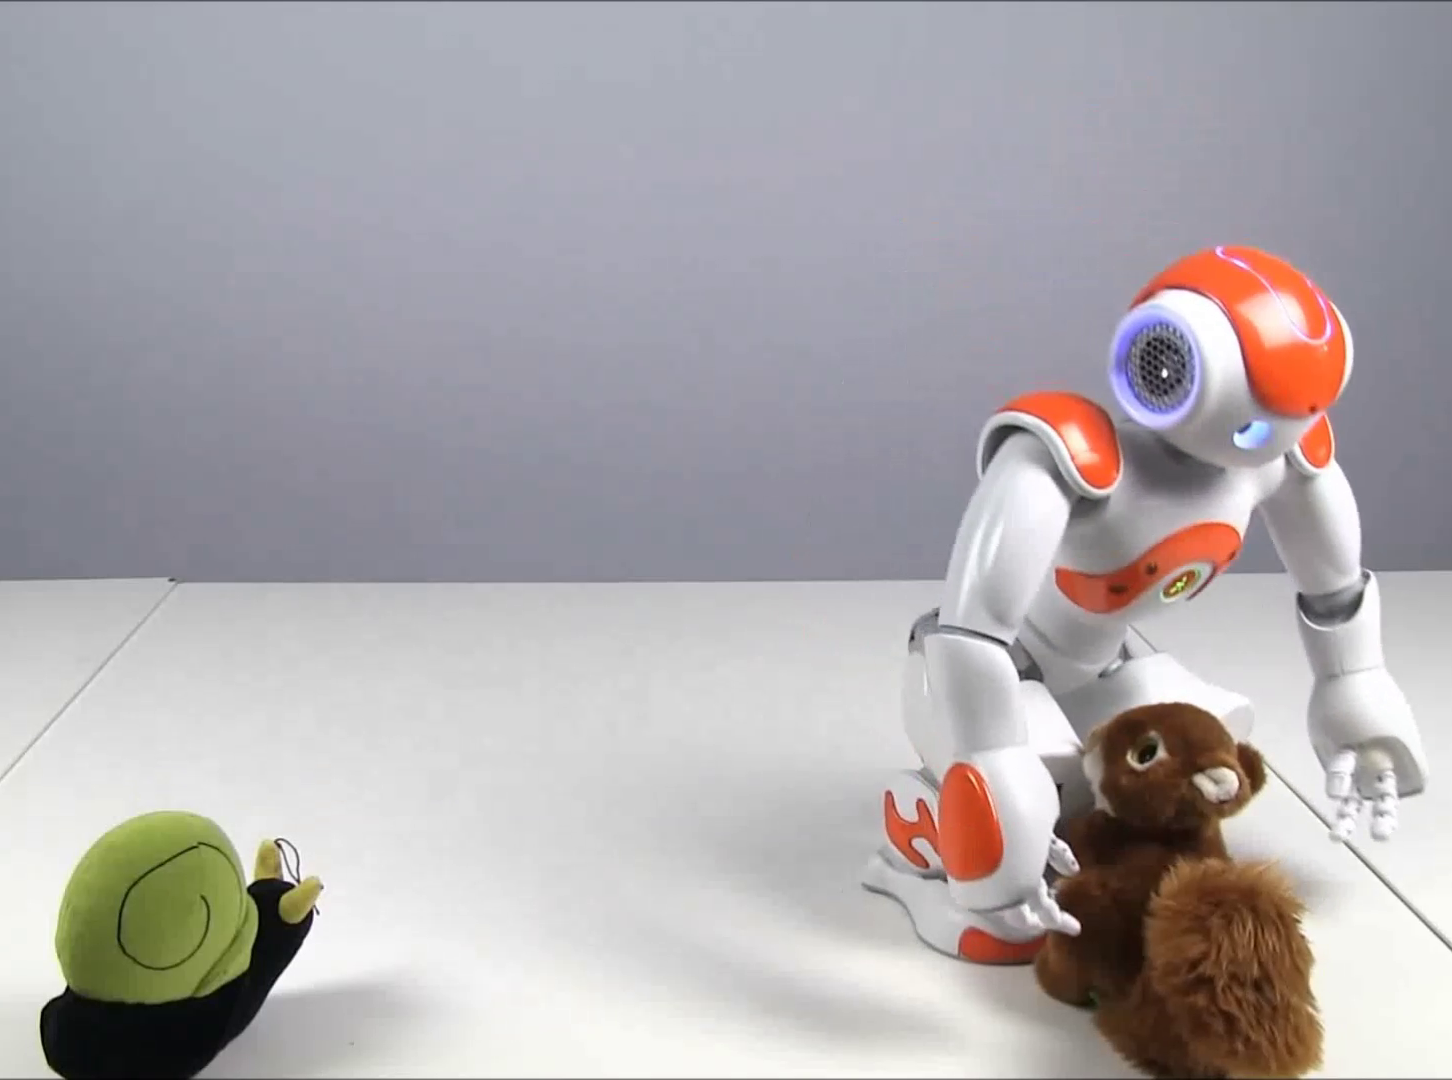
\includegraphics[height=5cm]{stimulus-robot-toys}
    }
    \subfigure[\emph{Picking} task, human condition]{
        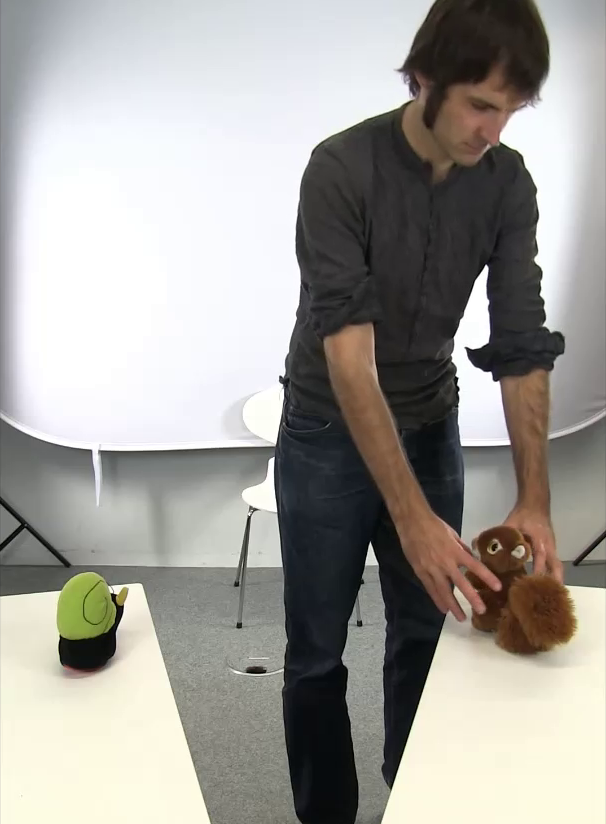
\includegraphics[height=5cm]{stimulus-human-toys}
    }

    \subfigure[\emph{Sound} task, robot condition]{
        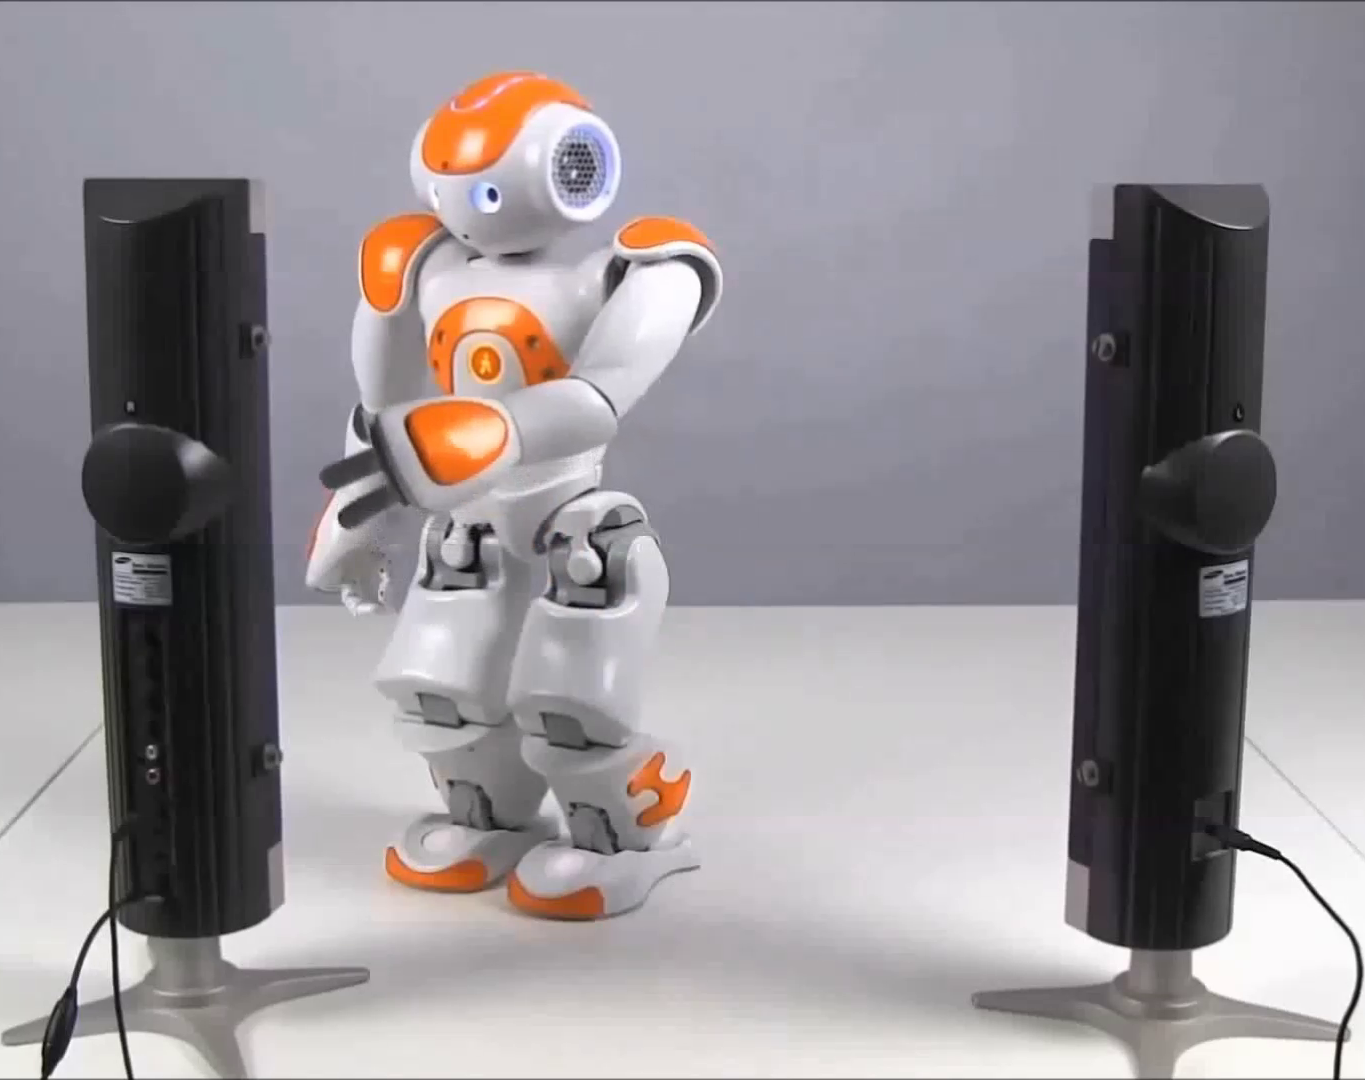
\includegraphics[height=5cm]{stimulus-robot-noise}
    }
    \subfigure[\emph{Sound} task, human condition]{
        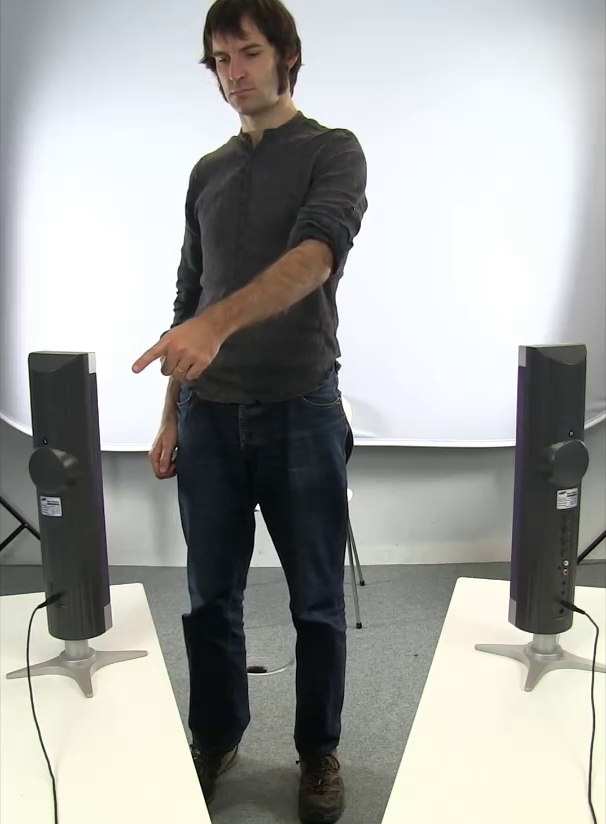
\includegraphics[height=5cm]{stimulus-human-noise}
    }


    \caption{\small Screenshots of the 2x2 stimuli. Note that the images above have been
    slightly cropped: the original video are framed so that the agent (robot or
    human) always remains entirely visible.}
    \label{fig:stimuli}
\end{figure}

\subsection{Questionnaires}

Before starting the experiment, the participants were asked to fill a
questionnaire which had 49 questions. The responses to the questions were scaled
in the 5-point Likert scale, numerically ranging from -2 to 2. The questionnaire
had ten questions from the 10 item big-five personality questionnaire. And then
there were questions taken from Godspeed questionnaire and other
questionnaires. In this report, we refer to this questionnaire as the
pre-questionnaire \ie before the experiment, and it typically took 5 minutes for
participants to fill it. 

A second questionnaire was administered at the end of the experiment, that was
almost identical to the pre-questionnaire.  This questionnaire typically took 3
to 4 minutes to fill and we refer to this as the post-questionnaire.

The difference (noted \deltaant, computation detailed below) observed for
each participant between the pre- and post-questionnaires form the dependent
variable of our experiment. It reflects the impact of the video stimuli on the
anthropomorphic perception that they have of robots \emph{in general}: the
Godspeed questions used in the questionnaires are not specific to the Nao robot,
and assess in a broader way how humans perceive robots.

\section{Experiment}

\subsection{Course of the study}

\subsubsection{Participants}

We ran first a pilot study with 10 participants, followed by an experiment with
57 subjects (mean age: 20.9, $SD=3.9$, 32 females and 25 males).

The participants were recruited amongst students of our university. To avoid
students with a high familiarity with robots and artificial intelligent systems,
Computer Science and Electronics curriculum were excluded. This was \textit{a
posteriori} comforted as per the questionnaire responses: no participants
reported itself as being very familiar with robots, 8 reported some familiarity
and 7 out of 57 own a domestic robot (vacuum cleaner).

The study lasted about 15 minutes per participant; each participant was invited
for one session only. Before leaving, each participant was given a reward
equivalent to EUR 10.

The study follows a 2$\times$2 design (table~\ref{table:design}): the
\emph{deep} vs {shallow cognitive context} condition was between-subject ( 31
subjects performed the \emph{deep cognitive} tasks while 26 were in the
\emph{shallow cognitive} condition); the \emph{robot} vs \emph{human} condition
was within-subject (the order of stimuli presentation was counter-balanced over
the 57 participants).

\subsubsection{Pre-questionnaire and familiarization}

\fxwarning{Was it first the pre-questionnaire or the familiarization?}
Before the experiment, participants were made to read, understand and sign a
standard consent form. Participants were then asked to fill the 49 questions of
the pre-questionnaire, without time constraint\fxwarning{right?}.

After the pre questionnaire, we invited the participants to an initial
free interaction with a \textbf{powered-off} Nao robot (we did not constraint
the time, and participants played between 2 and 3 minutes ith the robot).

The purpose of this pre-interaction was to get the participants acquainted with the
robot shape and kind of motions it could possibly perform, and therefore
mitigate the (visual) novelty effect (so that they do not get surprised seeing
a robot for the first time in the videos).

\subsubsection{Videos}

After filling the pre-questionnaire, we conducted a brief eye-tracker
calibration procedure, and the participants' gaze was recorded while they
watched the \emph{robot} and \emph{human} interaction videos.

\subsubsection{Post-questionnaire}

Finally, the participants were asked to fill the post-questionnaire.

\subsection{Data Collection}

\subsubsection{Gaze variables}

\paragraph{Areas Of interest}

Among the two scenarios, the first was one was about the robot/human picking up
a toy and the second one about pointing to the noise. As seen in
figure~\ref{fig:aoi}, we defined 10 areas of interest (AOIs): one on the head of
the agent (robot or human), two on the arms (left and right), two on the hands,
two on the legs and one on the torso. Besides, we defined one area of interest
per toy or speaker (depending on the stimulus).

\begin{figure}
    \centering
    \subfigure[\emph{Picking} task, robot condition]
    {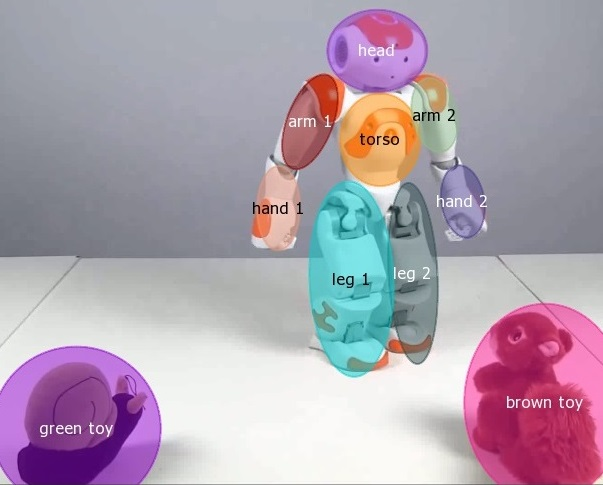
\includegraphics[height=5cm]{aoi-robot}\label{fig:aoi-toys}}
    \subfigure[\emph{Sound} task, human condition]
    {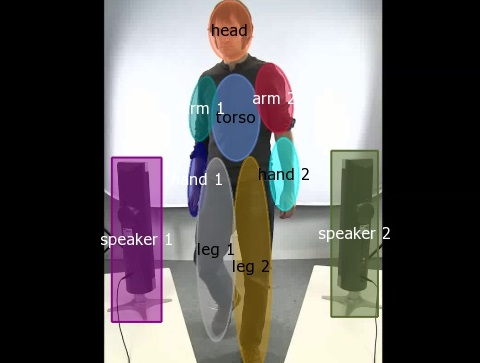
\includegraphics[height=5cm]{aoi-human}\label{fig:aoi-noise}}

    \caption{Areas of interest used for the gaze analysis}
    \label{fig:aoi}
\end{figure}

We collected the gazes falling into one of these 10 zones and analyzed
their distribution (producing what we call \emph{gaze patterns}).

\paragraph{Difference in gaze patterns}

An important data to be obtained here is $\delta_{\mathcal{H},\mathcal{R}}$. This is calculated by
taking the difference between the ratio of net dwell time on an AOI and the AOI
fixation coverage summed over all the AOIs in the scene. Hence,
$\delta_{\mathcal{H},\mathcal{R}}$ is expressed as a ratio in the range of 0 to
1. Similarly, the differences between gaze patterns of two participants, where
one watches the LC task, given by $\delta_{shallow}^{\mathcal{H},\mathcal{R}}$ and
the other watches the HC task, given by
$\delta_{deep}^{\mathcal{H},\mathcal{R}}$ are important gaze variables.

\subsubsection{Questionnaires processing}

\fxnote{TDB}

Questionnaires were coded and two values, the \emph{initial tendency to
anthropomorphize} \anti and the \emph{final tendency to anthropomorphize} \antf
were computed, respectively from the pre- and post-questionnaires.

These values were computed by a direct sum of the rating provided by the
participants for the Godspeed's questions in the category
\emph{Anthropomorphism} and \emph{\fxwarning{?}...}. These ten questions were
rated between -2 and 2, hence \anti and \antf vary between -20 and 20.

The other questions (including the Big-Five personality test) were not used for
this study.

\section{Results}

Based on the experiments conducted on 57 participants in the human
($\mathcal{H}$) and robot ($\mathcal{R}$) interactions across \emph{shallow} and
\emph{deep cognitive context} conditions, we have the following results. (the
detailed statistics and code used for obtaining the results are available here :
\url{https://github.com/chili-epfl/anthropomorphism-eyetracking})

\subsection{General Biases}

While testing for all the 4 hypotheses, we observed no significant bias with
respect to age, gender, EPFL status, familiarity with robot and robot ownership
of the participants, \ie there was no correlation found between these factors
and the gaze patterns in the videos.

\subsection{Manipulation check}

\begin{figure}
    {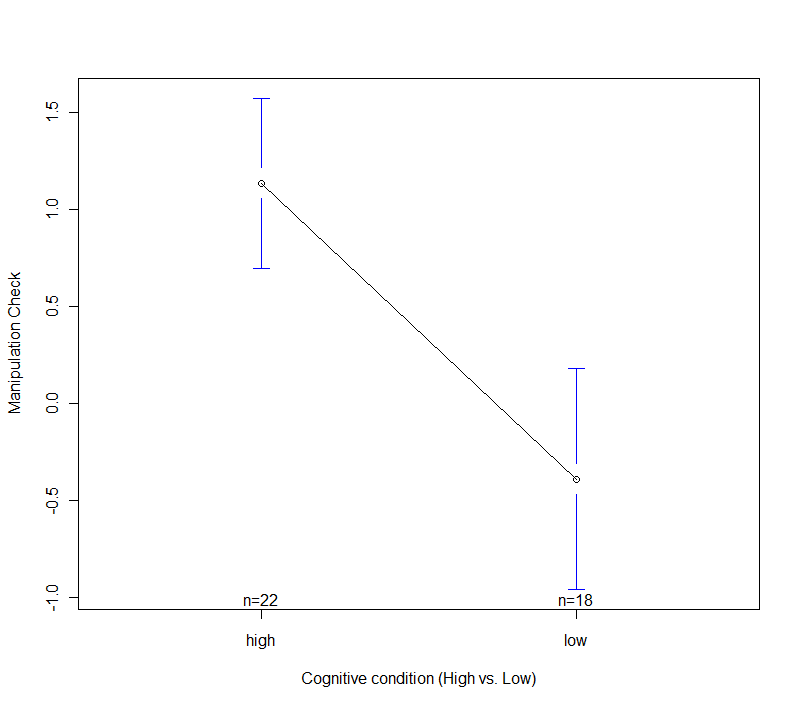
\includegraphics[width=3.3in]{ManipulationCheck}}
    \caption{Manipulation check}
    \label{fig:ManipulationCheck}
\end{figure}


In our post-questionnaire, we had a question asking the participants about
whether the video has a robot kind of task or a human kind of task on a scale of
-2 to 2 where -2 refers to robot kind of task. As can be seen in figure 2, we
got a significant correlation in this manipulation check ($F[1,36] = 20.42, p <
.01$) which means that the participants that were shown the \emph{shallow
cognitive context} videos identified the task as more robot-like and
participants watching \emph{deep cognitive context} videos perceived the tasks
as more human-like. 


\subsection{H1: Gaze differences between human and robot conditions}

We grouped the 8 areas of interest located on the agent into 4 categories : {\sf
head}, {\sf arm} (containing both arms and hands), {\sf torso}, {\sf leg}
(including both legs). And this is the result that we obtained from the ANOVA
between gaze patterns on the AOIs versus the human and robot videos :

{\sf head}: the fixations on the head for the human video
were observed to more than that for the robot video ($F[1,36] = 6.60, p < .05$)

{\sf arm}: the fixations on the arms for the $\mathcal{H}$ video
were also greater than that for the robot video ($F[1,36] = 18.65, p < .01$)

{\sf leg}: the fixations on the legs were much lower
for the human video as compared to the robot video ($F[1,36] = 2.89, p < .1$)

{\sf torso}: the fixations on the torso was more for the
human video than for the robot video ($F[1,36] = 3.54, p < .1$) 

\subsection{H2: Interaction between \anti and gaze patterns}

We got a significant correlation between $\delta_{\mathcal{H},\mathcal{R}}$ and
the \anti. As can be seen in figure 3(a), there is a significant negative
correlation between the two quantities (Pearson Correlation Coefficient = -0.42,
p < .01).

\begin{figure}
    \subfigure[Difference in gaze patterns vs \anti]
    {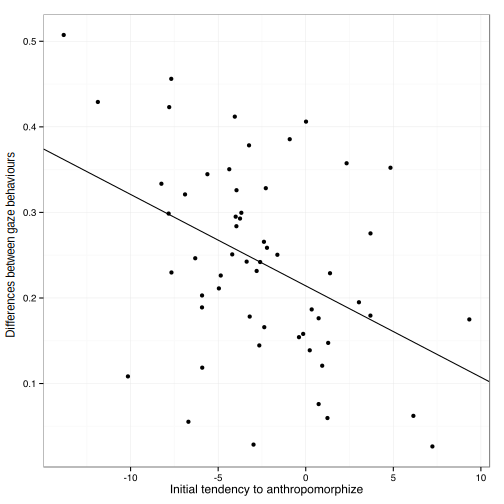
\includegraphics[width=3.3in]{H2}\label{GazeDifference-vs-ICA}}
    \subfigure[Gaze patterns for high vs low condition]
    {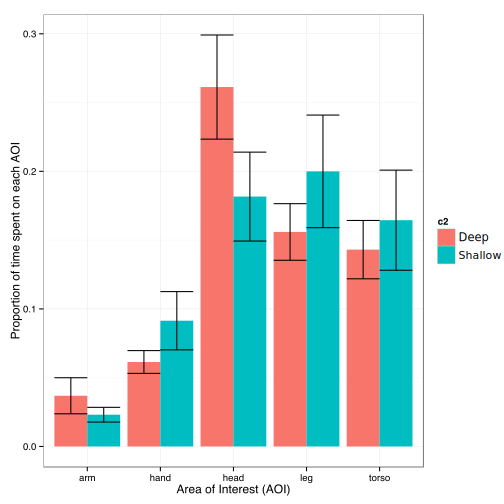
\includegraphics[width=3.3in]{GazeHighLow}\label{GazeHighLow}}
    \subfigure[Difference between \anti and \antf versus High/Low]
    {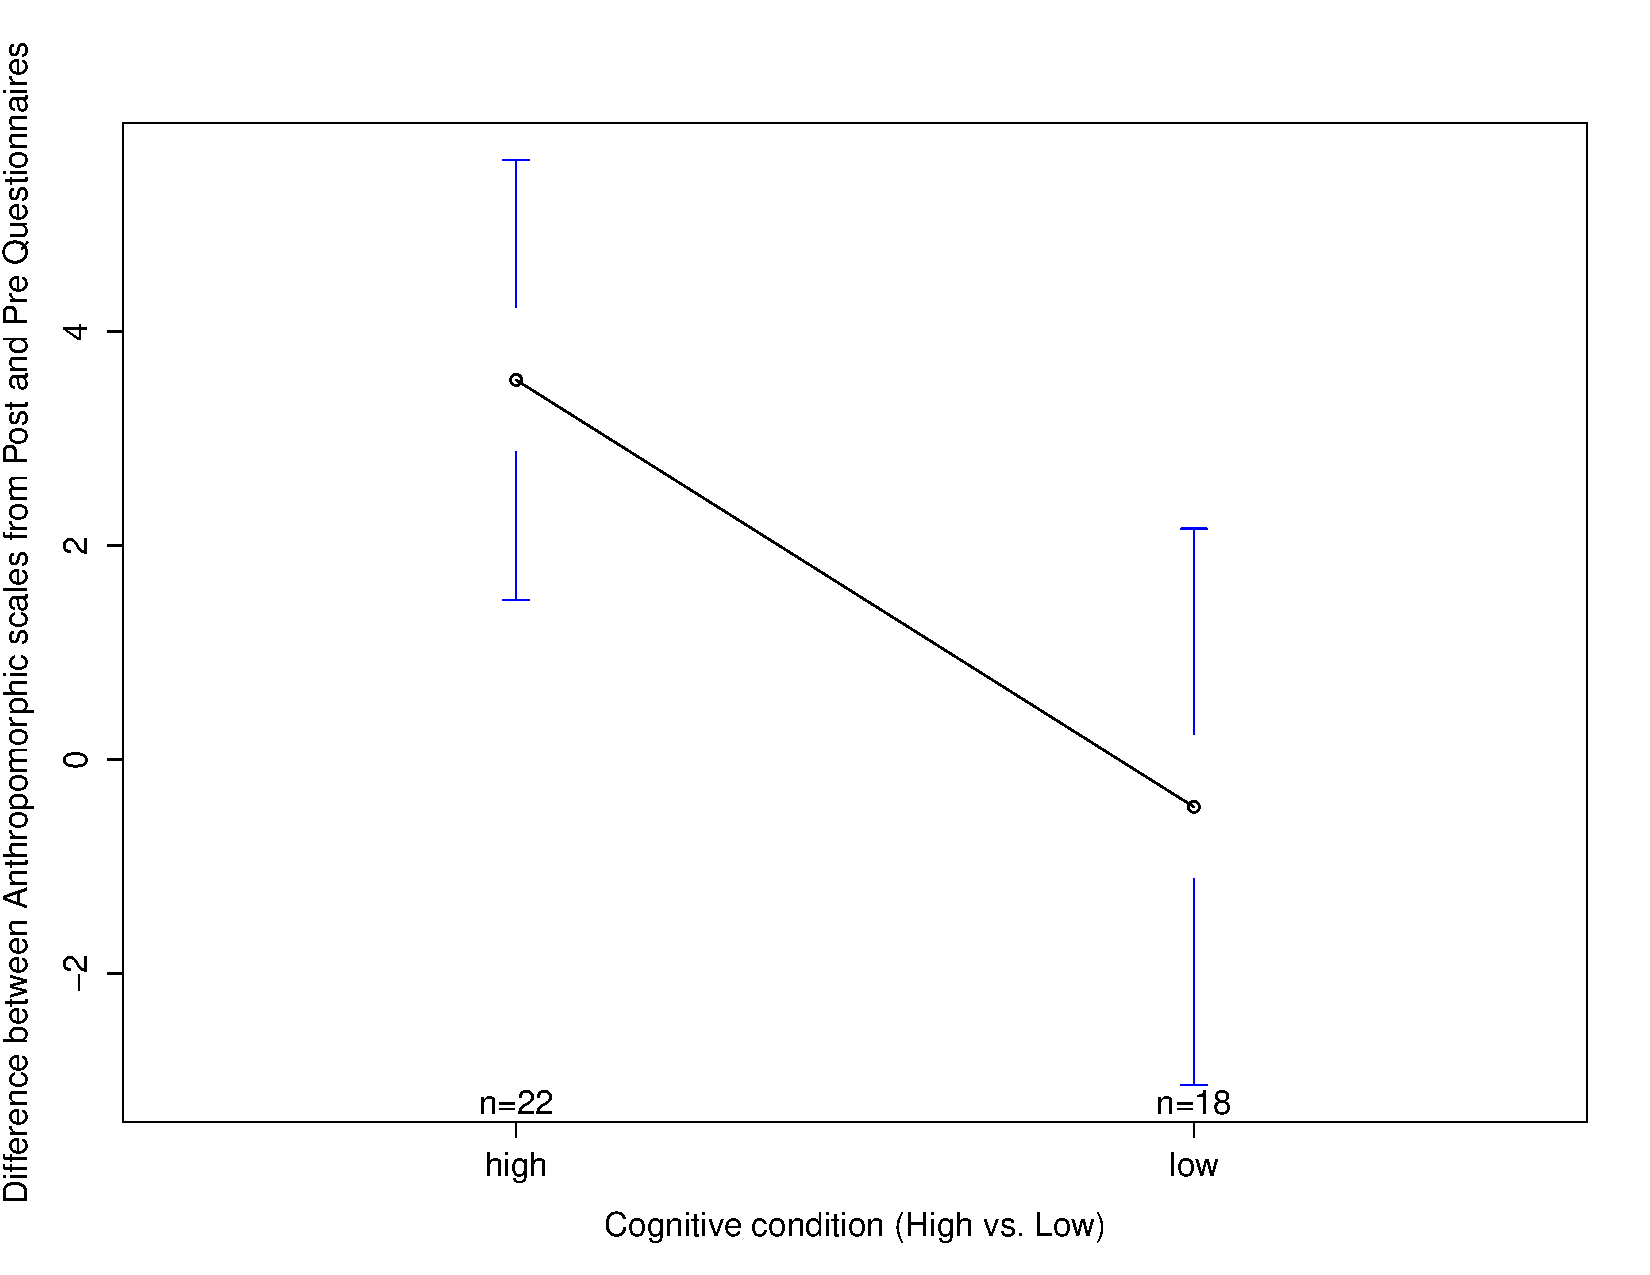
\includegraphics[width=3.3in]{H4}\label{ICAtoAAPImprovement}}
    \caption{Hypotheses H2, H3, H4}
\end{figure}

\subsection{H3: Gaze patterns for high vs low cognitive condition}

This test was done only for robot scenario as the human case is
by default a source of HC condition, hence, would not make a big impact in
changing the patterns across the LC and HC conditions. Based on ANOVA results,
taking just the 5 AOI groups (head, arms, hands, torso, legs) for the robot in
both LC and HC conditions, the fixations on the head in the HC condition was
found to be significantly higher than that in the LC condition (F[1,36] = 4.55,
p < .05). For all other AOI groups, the fixations across LC and HC were almost
the same. Figure 3(b) shows the distribution of proportion of time spent gazing
on the 5 AOIs for LC and HC conditions.

\subsection{H4: Difference between \anti and \antf versus High/Low}

ANOVA between \deltaant and the category of cognitive task
\ie HC or LC tells us that \deltaant is greater for HC tasks
than that for the LC tasks (F[1,36] = 6.54, p < .05). The results are shown in
figure 3(c).


\section{Discussion}

Based on the results that we obtained, we can now verify our four hypotheses.
For the first hypothesis where we state that the gaze patterns can distinguish
between human and robot interaction scenarios, we get greater
amount of fixation on the head, arms and torso for the human scenario as
compared to the robot scenario. This can be explained by the fact that
human is by default perceived as a high cognitive agent compared to a robot.
Hence, the proportion of time spent on looking at the head is more in case of
human videos as compared to robot videos. But the trend is opposite for legs.
This might be explained by the fact that the participants are fascinated by the
joints on the robot's legs \ie the novelty effect. Overall, this
result weakly validates our hypothesis.

In the second hypothesis, where we claim that $\delta_{\mathcal{H},\mathcal{R}}$
should correlate with the participants' \anti, we obtain in our results, a
significant negative correlation between the two quantities. From the negative
correlation, we can understand that if \anti is high, it means that the
\textit{human likeliness ascription} (HLA) is high (which means that there is a
greater tendency to anthropomorphize) which indicates that
$\delta_{\mathcal{H},\mathcal{R}}$ should be low. This supports our hypothesis
and can be explained by the fact that if HLA is high for a participant, then
even the robot videos are quite human-like for such participant. 

The third hypothesis where we state that the gaze patterns can distinguish
between HC and LC tasks, can also be supported by our results. As can be seen in
figure 3(b), the proportion of time spent by participants on looking at the head
is significantly higher in HC task as compared to LC task. When participants
ascribe more anthropomorphic features to robot, they look more at the head than
when they ascribe less anthropomorphic features.

Finally for the fourth hypothesis where we state that the cognitive priming will
have an effect on \deltaant, as seen in the results, \deltaant
for participants that watched the HC task is greater than that for the
participants who watched LC task. This proves the fact that HLA was induced by
the videos and in fact, the HC tasks impose a greater HLA on the minds of
participants than the LC tasks. This shows the typical priming effect of the
audio command given in the beginning of the video and highlights the variation
in HLA based on the interaction scenario (LC versus HC) thereby supporting our
hypothesis. 

We analyze the gaze distribution in this study only based on the AOI net dwell
times . Apart from this, the gaze transition among AOIs can be another way of
fetching gaze patterns which is not used in this study.

%%%%%%%%%%%%%%%%%%%%%%

No correlation between delta opinion and gaze fixation on head: are we measuring
two different things? or hidden variable?

If different things, then, gaze is possibly a better metric: in-the-moment, does
not suffer post-hoc reconstruction.

%%%%%%%%%%%%%%%%%%%%%%

\section{Conclusion}

In our experiment, we created two kinds of scenarios each for human and
robot interaction and just by changing the audio commands (priming
effect), we replicated these videos to create a HC and a LC scene. We recorded
the gaze patterns of the 57 participants who were made to watch these videos and
also the participants were asked to fill two questionnaires before and after the
experiment. These data were analyzed and compared to our four hypotheses. We
hypothesized that one who anthropomorphizes more would have a similar reaction
to human and robot conditions, and also that in the HC case, a
participant's fixations would be more on the head of the actor as compared to
that in the LC case. We also hypothesized that the HC scene would induce more
anthropomorphic attitude than the LC scene. We found that the results were
successful and supported our hypotheses. We also had another scenario where the
robot/human was asked to move/dance, but this scenario had only one object
(\ie the actor) showing movements, and hence participants would focus
more on seeing the movements leaving behind the cognition aspect, which made it
difficult to differentiate between the LC and HC cases and, therefore, we
discarded this scenario from our analysis.

\subsection{Context and Interaction Design}

\fxwarning{discuss here how context can be used to shape the interaction}


Anthropomorphism as a proxy for cognitive/affective bonds that are esthablishing
between humans and robots.

\fxnote{discuss extensions towards mobile eyetrackers}

\bibliographystyle{apacite}
\bibliography{biblio}

%\appendix
%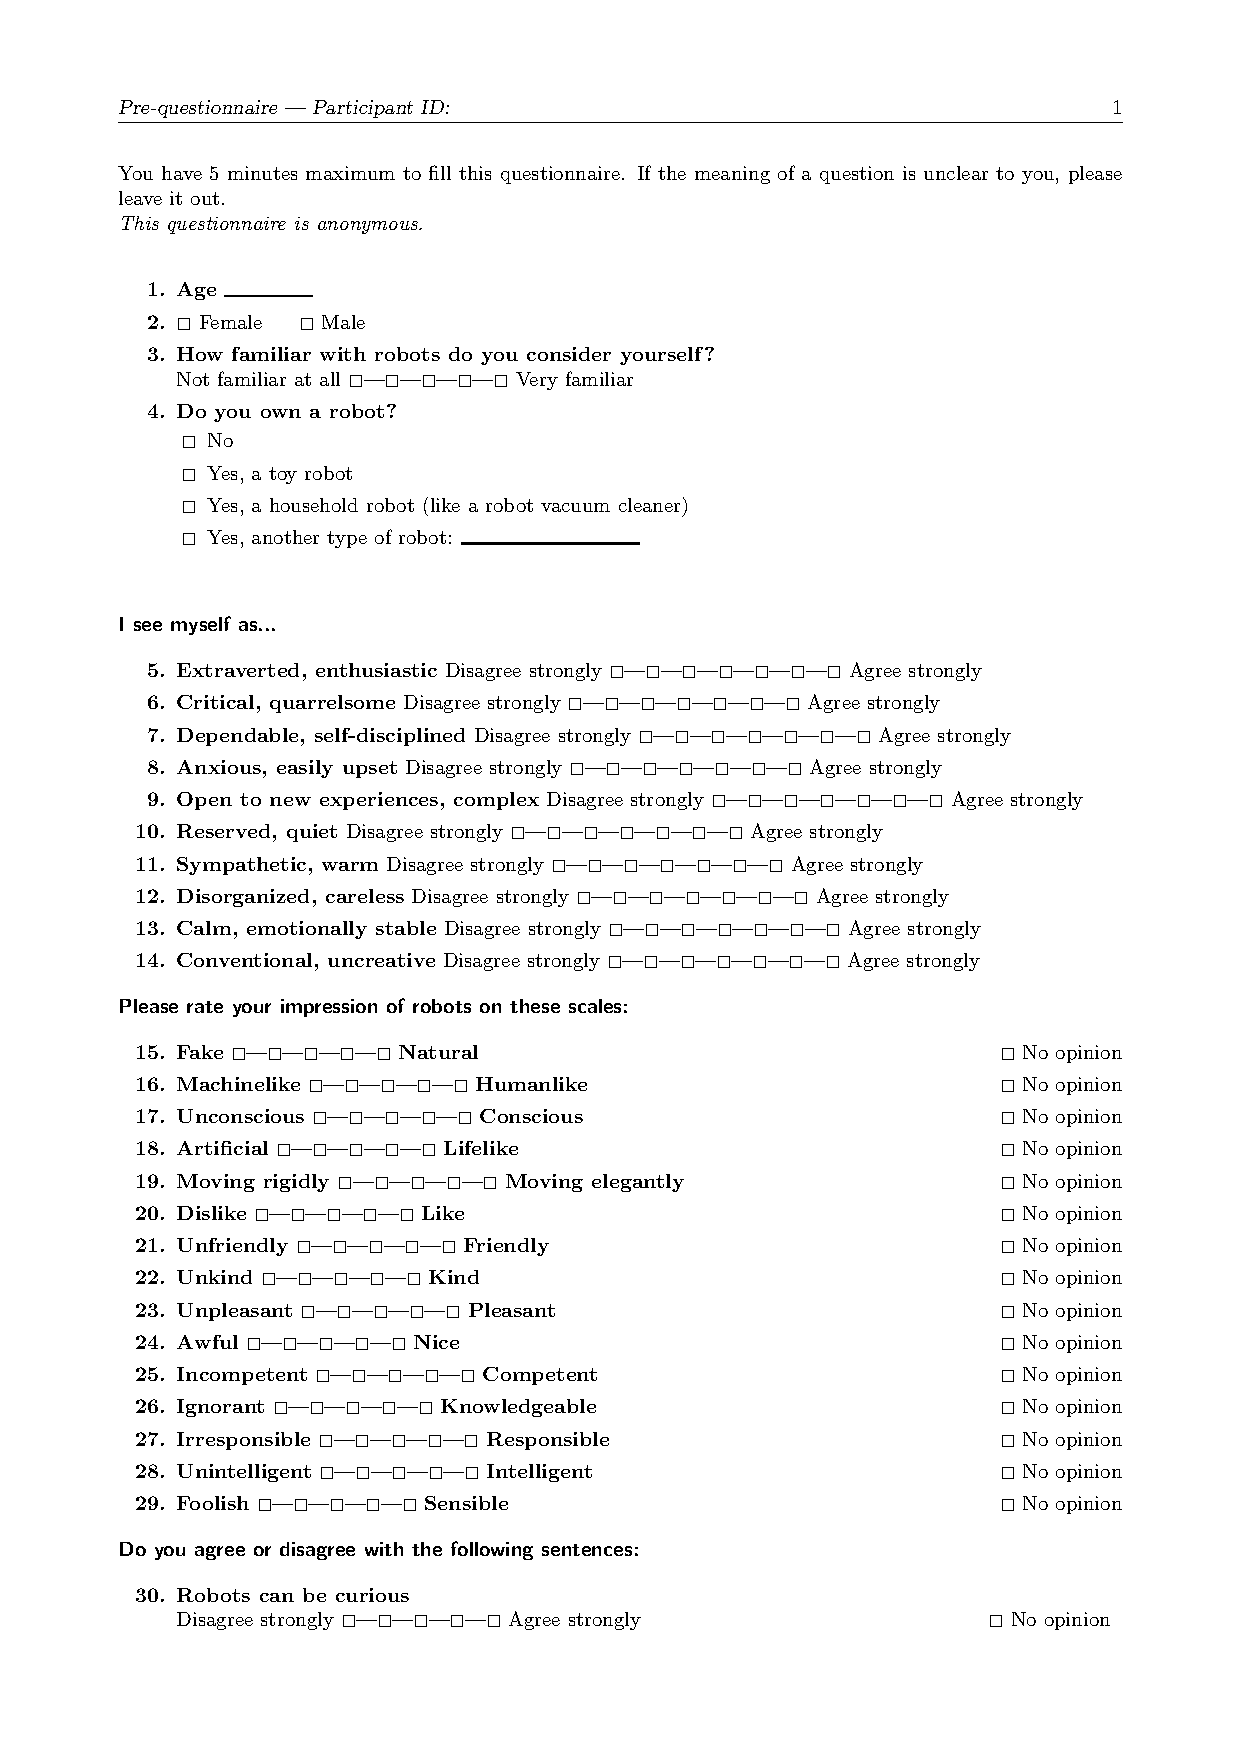
\includepdf[pages={1,2}]{pre-questionnaire.pdf}
%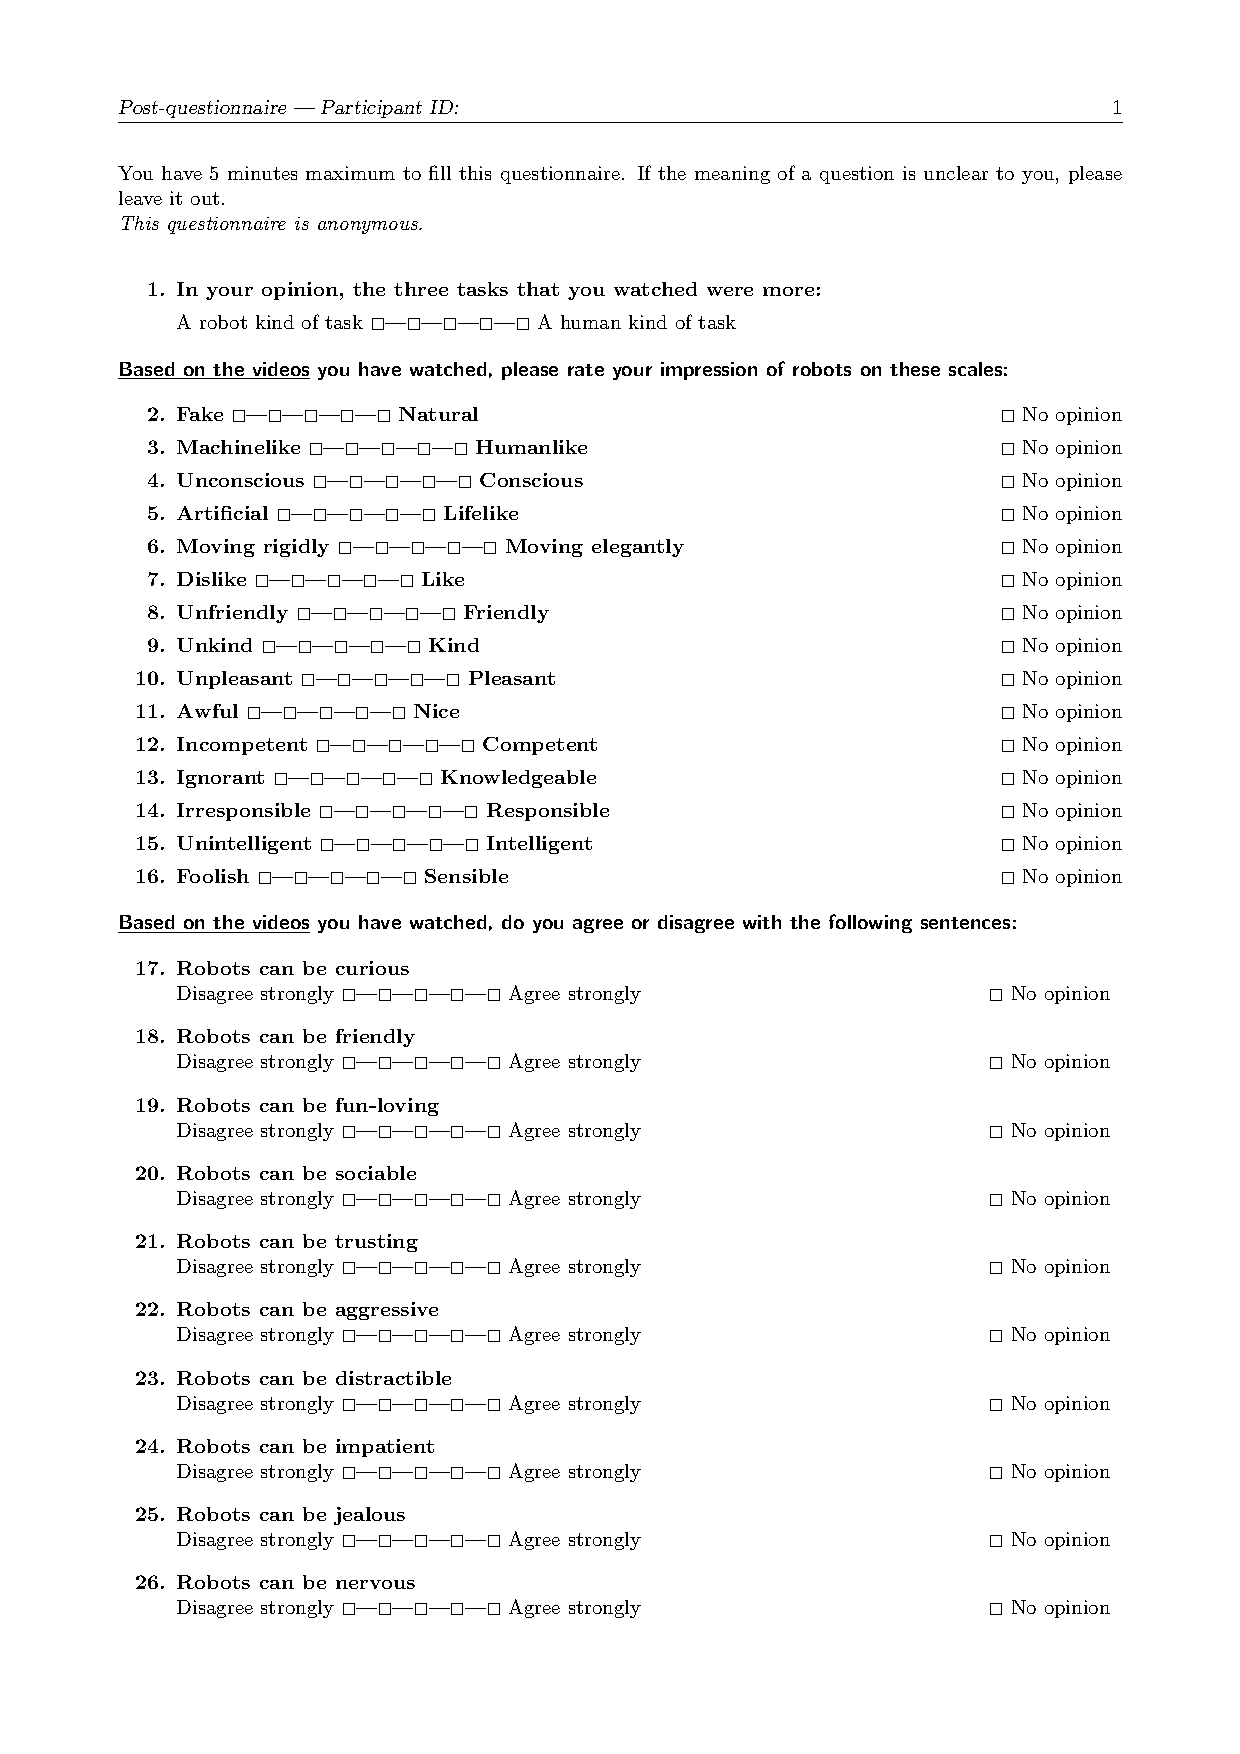
\includepdf[pages={1,2}]{post-questionnaire.pdf}

\end{document}
